%%%%%%%%%%%%%%%%%%%%%%%%%%%%%%%%%%%%%%%%%%%%%%%%
%
% start writing
%
%%%%%%%%%%%%%%%%%%%%%%%%%%%%%%%%%%%%%%%%%%%%%%%%

%%%%%%%%%%%%%%%%%%%%%%%%%%%%%%%%%%%%%%%%%%%%%%%%
%
% start writing
%
%%%%%%%%%%%%%%%%%%%%%%%%%%%%%%%%%%%%%%%%%%%%%%%%


\chapter{Literature study} \label{ch2_heading}

%\textbf{[Chapter introduction and context]}

To adequately answer the projects research question and test its hypothesis, a comprehensive understanding of the following topics needs to be established: i) Money laundering, ii) Complex network analysis for anti-money laundering processes, and iii) Machine learning approaches applied to an anti-money laundering context. Therefore, the chapter aims to give necessary background information on the topics mentioned earlier and investigate research that has already been conducted in these fields.        
\section{Financial crime - Money Laundering}

It is essential to understand money laundering and its known forms before thinking of how anti-money laundering processes can be improved. In short, money laundering is the process of making money that has been generated through illegal or criminal activities seem legitimate by misleading that the money launderer obtained the money in legitimate ways \citep*{buchanan2004money}.  \citet*{mcdowell2001senior} explained that the money laundering process contains three steps:

\begin{enumerate}

\item \textit{Placement}:  The process of placing illegal funds into financial institutions through wire transfers, deposits, or alternative means. 

\item \textit{Layering}: The process of separating the funds by performing a series of financial transactions that obscure the funds' origin.    

\item \textit{Integration}: The process of reintegrating the funds with formal sector economic activity. 

\end{enumerate}    

\citet{buchanan2004money} explained similar steps regarding the money laundering process. However, she provided additional information: The laundering mechanism is most vulnerable during the placement step because usually, money generated from unlawful activities takes the form of paper money, which is often difficult to conceal in large amounts. Therefore, money launderers carefully need to establish ways to introduce large amounts of cash into the financial system incrementally. Money launderers commonly use front corporations to deposit cash or cashing businesses to convert cash to financial instruments such as money orders, traveller's checks, and cashier checks. The layering step aims to construct a complex web of transactions representing legitimate financial activity based on the transactions' volume, frequency, and monetary value. If the layering is complete, it is challenging to reconstruct a paper trail. Also, offshore financial institutions play an essential role in the layering step. Finally, regarding the integration step, standard financial instruments used to reintegrate the ``washed'' funds are bills of lading and guarantees, banknotes, bonds, and letters of credit.   	      

The essence of the money laundering process is encapsulated within the steps mentioned above. However, these steps are executed using different money laundering tools and techniques. For example, \citet{buchanan2004money} explained that there are seven tools or techniques most commonly used by money laundered that help them successfully launder money. These techniques are:

\begin{enumerate}

\item \textit{Structuring}: A person is known as a ``smurf'' when they intentionally avoid reporting financial transaction requirements by making deposits that are less than the country's prescribed threshold. In South Africa, this threshold is defined in the FIC act that states that all institutions are obligated to report on cash transactions bigger than the prescribed threshold. According to the financial intelligence centre, the prescribed threshold limit in South Africa is R24 999,99 \citep*{fic2001}. Money launders deposit large amounts by breaking them up into increments less than the prescribed limit and depositing these increments from different accounts. As a result, money launderers avoid reporting the requirements of cash transactions to authorities. The prescribed threshold may vary from country to country. For example, the prescribed threshold in the US is \$10 000 \citep*{yale2021reporting}.        

\item \textit{Front companies}: Front companies are considered to be an effective money laundering tool for two reasons: i) front companies do not necessarily require the collaboration of financial institutions and, ii) detection of criminal activity within front companies that are conducting legitimate business is challenging (especially when the front company is exempt from any currency transaction reports). Businesses that commonly function as front companies are cash-rich, for example, liquor stores, restaurants, cheque cashing businesses, and travel agencies. Also, companies that import and export goods can function as front companies. These companies launder money by double invoicing, over/undervalued goods, inflating prices for imported goods, and financial exports.

\item \textit{Trade misinvoicing}: This is a widespread money laundering technique that involves the misinvoicing of international trade transfers. Trade misinvoicing involves illegally moving money across borders by deliberately falsifying the type of commodity, its volume, and its value in an international commercial transaction. For example, consider the scenario where criminals used company X, a precious metals front company, for trade misinvoicing. Company X can create falsified invoices for importing gold from Peru. As a result, illicit funds can be transferred to Peru. Trade invoicing is very dangerous since criminals can transfer substantial sums of money across international borders.  

\item \textit{Shell companies}: According to the Financial Action Task Force, a shell company is defined as an institution ``that does not conduct any commercial or manufacturing business or any other form of commercial operation in the country where their registered office is located.'' Shell companies are often established in countries where offshore financial centres are characterised by: no or low taxes based on business income/investment, looser tax codes, strong bank secrecy, and no need for the physical presence of financial institutions, corporate or legal entities within the jurisdiction in question. Examples of offshore financial centres are Panama, the Bahamas, the Cayman Islands, and the Netherlands. The volume of transactions and secrecy laws of the offshore financial centres make it nearly impossible to investigate potential money laundering instances.   

\item \textit{Correspondent banks}: Correspondent banking has recently raised severe money laundering concerns. Correspondent banks are banks situated in a country to provide services for another bank or financial institution in a foreign country. Figure \ref{fig:ch2_correspondent_bank} gives a visual illustration of the relationship between the banking clients, domestic banks, and correspondent banks and tries to convey the core idea of when money gets wired across different jurisdictions. The risk for the money laundering process arises due to differences in anti-money laundering compliance programs between the foreign and domestic banks (originator A's and beneficiary B's domestic banks, see Figure \ref{fig:ch2_correspondent_bank}). It is possible that a foreign bank's anti-money laundering compliance program is not sufficient to meet the anti-money laundering requirements of a domestic bank.

% FCH2_1 - Correspondent bank
\begin{figure}[h]
	\begin{center}
		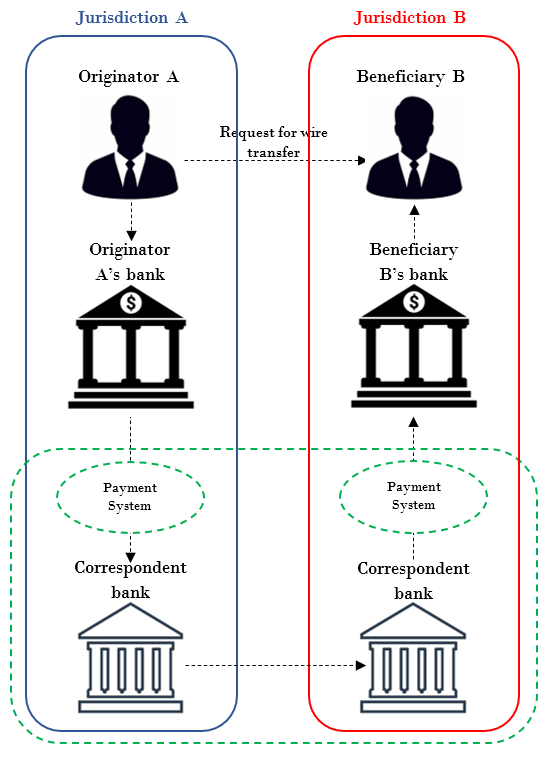
\includegraphics[width=8cm]{fig/CH2/correspondent_bank_01.png}
		\caption{The arrows dictate the flow of information between the entities in the diagram. The role of corresponding banks can be explained as follows. Originator A would want to wire transfer money to beneficiary B. Originator A will log this request with their domestic bank (acting as a responded bank). Originator A's bank will then log the transaction request with the correspondent bank. As a result, the correspondent bank, which has both jurisdictions, can transfer the funds to beneficiary B's domestic bank. Beneficiary B's domestic bank (also acting as a respondent bank) will then make the funds available to beneficiary B.}
		\label{fig:ch2_correspondent_bank}
	\end{center}	
\end{figure}
   
\item \textit{Mirror trading}: The non-fraudulent meaning of mirror trading is when a forex or stock trader mimics the trading strategy of experienced brokers \citep*{chen_2021}. The recent incident with Deutchbank in 2017 obscured the meaning of mirror trading.  The fraudulent meaning of mirror trading is when an individual that owns two accounts buys contracts for one account while selling an equal amount of contracts from the other. The incident with Deutsch bank will be used as a motivating example. A Russian customer of Deutsch bank bought securities against ``Russian Ruble'' from Deutsch bank in Moscow. Simultaneously, a non-Russian customer of Deutsch bank sold the same number of securities to Deutsch bank in London in exchange for US dollars. Unfortunately, Deutsch bank failed to connect the two customers working together at this scheme. As a result, mirror trading (the fraudulent type) was used as a tool to move funds (Russian Ruble) out of Russia and into other jurisdictions and currencies (US dollar). 

\item \textit{Parallel banking systems}: There is a possibility that illicit funds never enter mainstream financial systems. Instead, criminals use underground banking systems (parallel banking systems) to launder money. Examples of parallel banking systems are Hawala and Hundi systems in India or the Chop or fei chi in China. The basic idea behind these parallel banking systems are as follows: i) a person can deposit money in exchange for some marked object (chip, ticket, etc.) which is impossible to replicate; ii) a person can exchange the object for its monetary value in another country (in paper cash); iii) upon exchange, the person pays a commission fee (typically 5-15 percent of the original amount). The exact functioning of these parallel banking systems is unknown. Experts say that these systems can range from being extremely complex to being very simplistic \citep*{schramm2003evolution}. These parallel banking systems are ideal for money launderers since there is little or no documentation about the events, and no funds will cross borders. The challenge for regulatory authorities is to be vigilant for indications that suggest that parallel banking systems are present. 
\end{enumerate}

Now that a preliminary understanding of the problem - money laundering and its components have been established, the paper can shift its focus towards the solution - anti-money laundering. As mentioned in the introduction of the paper, anti-money laundering refers to the regulations, procedures, and laws intended to prevent criminals from obtaining legitimate funds generated by illicit activities. The history of anti-money laundering dates back to the 1970s when legislation started to develop. In 1989 the fight against money laundering intensified with establishing the Financial Action Task Force (FATF). The FATF resulted from a group of countries that came together to investigate and construct anti-money laundering measures, establish international anti-money laundering standards, and promote adequate implementation thereof. Various anti-money laundering regulations are imposed on financial institutions due to their vulnerability to the crime. Therefore, anti-money laundering legislation and regulations ensure that financial institutions have adequate anti-money laundering processes. 

\citet*{sudjianto2010statistical} provided an overview of a general anti-money laundering process, see Figure \ref{fig:ch2_aml_process}. The first phase of anti-money laundering is the customer screening phase. This phase evolves, enforcing the \textit{Know Your Customer Policy} and implementing an \textit{Enhanced Due Diligence} check during the account opening process. The Know Your Customer Policy is a set of standards used by financial institutions to verify customers personal profiles, risk profiles and financial profiles. The Enhanced Due Diligence check is primarily done to check the customer's identity. The information gathered from the Know your Customer and Enhanced Due Diligence check is processed by a risk rating model (an inference model or rule-based model) to output a risk score, which indicates the potential customer's risk. The second phase of the anti-money laundering process continuously monitors customer transaction activity. \citet{sudjianto2010statistical} explains that there are four steps in the customer transaction monitoring phase:

\begin{enumerate}
    \item \textit{Identify:} The focus of this step is to identify suspicious activity. The step entails observing if historically known suspicious activity occurs, surveillance of high-risk customers (identified in the first phase), and trying to detect emergent patterns that might indicate risky behaviour.     
    
    \item \textit{Prioritise:} The first step could generate false positives cases. Therefore, the goal of the prioritise step is to prioritise and rank cases that fraud experts should investigate later on.
    
    \item \textit{Investigate:} After prioritising suspicious cases, experts investigate these cases. The investigation requires intense human resource capacity and manual intervention, unlike the previous two steps. It is up to the expert to investigate and pull information from various sources to ``create a story'' for their investigation.    
    
    \item \textit{Report:} If a case is deemed suspicious, it needs to be reported for further investigation by law enforcement. A detailed report is needed for authorities to continue the investigation and promote learning. In addition, banking personal must make system updates to identify future cases with similar characteristics.    
    
\end{enumerate}

% FCH2_2 - AML process
\begin{figure}[h]
	\begin{center}
		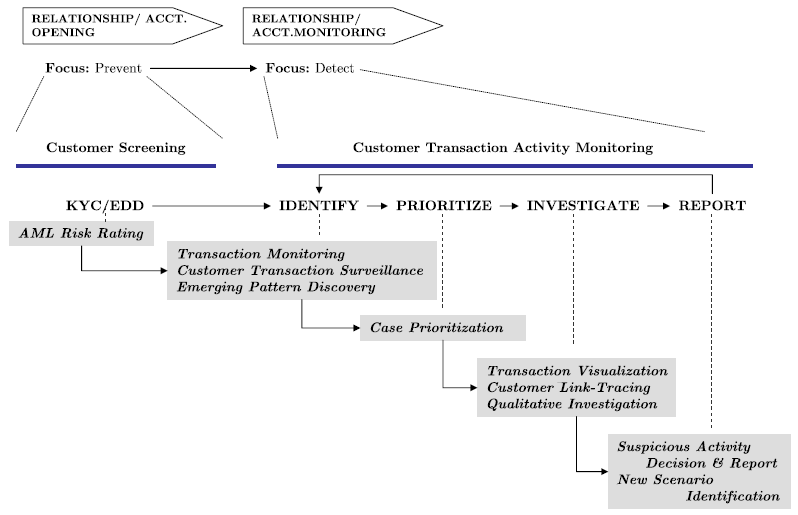
\includegraphics[scale=0.75]{fig/CH2/aml_process_02.png}
		\caption{The general anti-money laundering process as described by \citet{sudjianto2010statistical}. The process consists of two phases, customer screening and customer transaction activity monitoring. The first phase enforces the Know Your Customer (KYC) policy and performs an Enhanced Due Diligence check (EDD). The second phase consists of four steps, i) identify, ii) Prioritise, iii) Investigate, and iv) Report.}
		\label{fig:ch2_aml_process}
	\end{center}	
\end{figure}

There are multiple stages and steps within the anti-money laundering process. The project will not attempt to improve the entire process. However, the project will attempt to provide evidence that might improve a subset of the process, specifically identifying and prioritising steps within the second phase of the anti-money laundering process. For example, in generating the network features, the project will use historical transactions (obtained by the customer transaction monitoring phase) to construct a client network. The network features with other useful client features are then presented to some learning algorithm that seeks to \textit{identify hidden patterns} (step 1, phase 2 of the general anti-money laundering process) within the data. After choosing the best-suited learning algorithm, a model is constructed, which provides  the probability that a banking client is engaged in money laundering activities. Therefore, high-risk clients can be \textit{prioritised} (step 2, phase 2 of the general anti-money laundering process) by ranking each client based on their obtained risk score.   

It would be interesting to understand how the identification and prioritisation steps (Figure \ref{fig:ch2_aml_process}) are executed by different banks. Unfortunately, the literature vaguely explains the details of current industry-standard anti-money laundering processes, specifically those geared towards identifying suspicious transactions/clients and their ranking. This information gap is understandable because financial institutions prohibit publications since they contain sensitive content. However, literature seems to indicate that most banks implement a rule-based approach in identifying suspicious transactions \citep{abdallah2016fraud, chen2018machine, sudjianto2010statistical, gao2007framework}. Unfortunately, the degree of complexity of the rule-based approaches is not mentioned. However, there is a consensus that rule-based approaches are predominantly implemented due to their ability to effectively filter through masses of client transactions.   

On the other hand, rule-based systems implemented in commercial banks experience the problem of not adapting their rules quickly enough to capture the dynamic behaviour of money laundering criminals. Trying to capture the dynamic behaviour of money laundering criminals is only one of the challenges the modern-day fraud detection systems need to handle. Literature details various challenges and issues that general fraud detection systems face \citep{abdallah2016fraud, sudjianto2010statistical, gao2007framework, van2017gotcha} . These challenges apply to banking fraud (credit card fraud and money laundering) and other fraud areas such as insurance fraud, telecommunication fraud, online fraud, etc.    

From the papers investigated, \citet{abdallah2016fraud} defined the most comprehensive set of challenges and issues that modern-day fraud detection systems encounter. These challenges are i) Concept drift, ii) Skewed class distributions, iii) Large amounts of data, and iv) Infrastructure for real-time detection. \textit{Concept drift} is described as a phenomenon in that the underlying model (or concept) changes over time \citep*{abbass2004online}. This phenomenon directly relates to the \textit{drift phenomenon concept}, described in the context of fraud detection systems, when the behaviour of fraudsters and legitimate users continuously changes \citep*{gama2014survey}. Concept drift is a tremendous challenge when statistical learning models are constructed since there is a possibility that the model is constructed using outdated data. Using outdated data is problematic because of the high likelihood that the relationship between variables considered in the model has already changed \citep{gama2014survey}. The second challenge mentioned by \citet{abdallah2016fraud} is \textit{skewed class distributions} or imbalanced classes. In fraud detection systems, skewed distributions are when the typical instances (for example, legitimate transactions) exceed the amount known fraudulent instances (for example, suspicious transactions) by a significant factor \citep*{maes2002credit}. Skewed class distributions, especially when the variable of interest is in the minority class, can cause problems with the learning algorithm (assuming that the detection system uses one). If there is not enough data for the learning algorithm, it will not discover patterns within the data \citep*{abu2012learning}. The third challenge fraud detection systems experience is with the \textit{quantity of data}. Often vast amounts of data need to be processed by fraud detection systems. The data introduced to fraud detection systems have high dimensionality, meaning that the data set contains multiple features/variables/inputs/attributes.  The colossal size of the data sets makes it difficult for fraud detection systems to process this information and, secondly, in a timely manner. The final challenge mentioned by \citet{abdallah2016fraud} is that fraud detection systems are challenged with \textit{supporting real-time detection}. Therefore, these detection systems should be designed to efficiently use their resources (time and memory) to detect illicit activity immediately.

The challenges mentioned by \citet*{van2017gotcha}, \citet{sudjianto2010statistical}, and \citet{gao2007framework} had some overlap with the above-mentioned challenges. However, they did have the following to add: \citet{van2017gotcha} added that fraud has the characteristic of being \textit{imperceptibly concealed}. In fraud detection systems, the term means that criminals expertly disguise themselves as honest clients in all possible areas (including the data). Therefore, defining what makes a client or transaction honest is the true challenge for any fraud detection system. \citet{sudjianto2010statistical} also added that in the case of a fraud detection system that utilises a statistical model, the problem of \textit{learning mislabeled classes} could arise. This problem occurs particularly with money laundering because most suspicious cases (reported by the anti-money laundering process) are evaluated externally. The result of these investigations are often not promising, and the financial institution rarely learns anything. Therefore, suspicious cases are easily mislabeled.

Providing a solution for each of the challenges mentioned above is beyond the project's scope. However, as mentioned in the introduction of the project, the project's objective is to provide evidence that incorporating network features into the feature set used as input to a machine learning model will enhance the performance of the  money laundering classifiers. Therefore, it is beneficial for the project to be aware of the challenges mentioned above and their mitigation strategies. The following section gives an overview of machine learning, a brief discussion of popular machine learning algorithms used in anti-money laundering processes, and examples of how machine learning is applied in an anti-money laundering context.  

\section{Machine learning approaches for financial fraud detection}.

\citet{abu2012learning} explains that there exist various views of what ``learning from data'' is. \textit{Statistics} is one of the fields that offers its view on the task. More specifically, statistics is concerned with probability theory and applying said probability theory in building \textit{models} which replicate the underlying data generating process. The statistician is thus conscious of the structure proposed for the underlying process and interprets at the hand of that structure. Another view of learning from data is the view presented by the \textit{data mining} discipline. Data mining is described as a practical field that focuses on finding anomalies, patterns, or correlations in large relational databases. Although the field of machine learning contains components of both these fields, it should be distinguished as a learning view on its own.
 
The field of machine learning is the main field dedicated to learning from data \citep{abu2012learning}. The basic premise of learning from data from machine learning's view is to utilise a set of observations to undercover underlying processes. This is a very broad premise, and although the premise is somewhat shared with statistics, the main difference  between machine learning and statistics lies in their approach. Machine learning is only concerned with \textit{predicting} what is generated by the underlying process and not establishing the underlying data generating process (as in statistics). For these purposes, machine learning relies on over-specified mathematical structures, for which the mappings are not easily interpretable, and careful application of probability theory in identifying a constrained configuration of said structure is useful for predicting observations. This being said, there are similarities between how both are applied. For example, both rely heavily on probability theory and mathematical models. Statistics results in more interpretable propositions for the relationship between inputs and outputs, whilst machine learning sometimes provides improved prediction performance at the cost of interpretability. Both the qualitative and quantitative objectives of the study dictate how useful and appropriate either may be. The judgment in this regard is at the discretion of the analyst. This project will use machine learning as one of the main components in (dis)proving its premise. 

From machine learning's view, it is difficult to encapsulate the broad premise of learning from data within a single framework. Therefore, as a result, different learning paradigms were developed to deal with the different situations and assumptions. The following basic notation needs to be established before listing and describing the different learning paradigms or types of learning. This notation was predominantly adopted from \citet{abu2012learning} and \citet*{et2020pien}.
 
A data set $\mathcal{D}$ contains $N$ observations each consisting of a response, denoted by $y_i$, and vector of features/predictors associated with the response variable denoted as $\{\boldsymbol{x}_i = [x_{i1},x_{i2},\ldots, x_{ip}]^T :i = 1,2,\ldots,N$\}. In the case where the response is \textit{multi-valued} then it will be denoted by $\{\boldsymbol{y}_i = [y_{i1},y_{i2},\ldots, y_{iq}]^T :i = 1,2,\ldots,N\}$, where $p$ and $q$ denote the input and output dimensions respectively. Furthermore, $f$ will denote a unknown target function, which describes the relationship between all possible input values (input space), denoted by $\mathcal{X}$, and their corresponding responses (output space), denoted by $\mathcal{Y}$. 

Now that the paper established the preliminary notation, it can further investigate the different learning paradigms. The two most popular learning paradigms or types of learning are \citep{abu2012learning,et2020pien, james2013introduction}:

\begin{enumerate}
    \item \textit{Supervised learning}: A supervised learning task aims to predict some response. This task involves using models and learning algorithms to extract a pattern from the data (i.e. finding a relationship between the predictors and responses). For example, suppose we have the predictors, $\boldsymbol{x}_i$ and their associate response, ${y}_i$. With a supervised learning task, the goal is to find a function that best represents $f$. As a result, responses can be predicted (given the predictors), and an understanding of the relationship between the response and predictor variables (inference) is established.  The process of approximating $f$ is referred to as training the model. This process is possible due to the learning methods ability to ``supervise'' its performance, hence, why the task is called ``supervised learning''.
    
    \item \textit{Unsupervised learning:} In contrast to supervised learning, unsupervised learning tasks are strategies for identifying structures in the data without the aid of a response variable. Therefore, for every observation $i$, we have a vector of measurement $\boldsymbol{x}_i$ but no associate response $y_i$. Therefore, the learning type is called ``unsupervised'' due to the absence of the response variable that acts as a supervised mechanism. Unsupervised methods aim to discover the relationship between variables or between the observations.
    
\end{enumerate}

The learning paradigms mentioned above are not the only learning types. Other types of learning include reinforcement learning, semi-supervised learning, self-supervised learning, multi-instance learning, etc. Although much research has been done in applying unsupervised methods in the financial fraud domain \citep*{al2021financial, salehi2017data, abdallah2016fraud} this project will focus on \textit{supervised learning} applied in an anti-money laundering context. 

There are two common types of supervised learning problems \textit{regression} and \textit{classification}. Regression is described as a supervised learning problem with a numeric or quantitative response and classification as a supervised learning problem with a categorical or qualitative response \citep*{james2013introduction}. The general formulation of supervised banking fraud problems (including money laundering) is formulated as a binary classification problem:

Given a data set ($\mathcal{D}$) with predictors $\{\boldsymbol{x}_i:i = 1,2,\ldots,N\}$ and response $\{y_i:i = 1,2,\ldots,N\}$, where:

$$y_i = \left \{\begin{array}{ll} 
 +1 &  \text{if observation is `fraudulent'},\\ 
-1 & \text{if observation is `non-fraudulent'. } 
\end{array} \right.$$

 let the chosen learning algorithm pick $g$, from the set of candidate formulas, known as the hypothesis set $\mathcal{H}$, such that $g$ approximates $f$ ($g \approx f: \mathcal{X} \rightarrow \mathcal{Y}$). 

The above formulation may be an over-simplification of how certain supervised banking fraud problems are formulated. However, it conveys the central idea of the problem setup. Also, most supervised banking fraud problems are formulated as classification problems \citep{al2021financial, abdallah2016fraud, salehi2017data}. Therefore, the project specifically focused on \textit{classification} applied in an anti-money laundering context.

\section{Network analytic's for fraud prevention} \label{ch2_sub_heading_network}

Networks are ubiquitous in nature. Physical networks such as highways, electric power grids, subway systems, etc., are easily identifiable, but \textit{abstract} networks are less tangible such as social relationships, biological systems, etc. Real-world networks, physical and abstract, generally are \textit{dynamic}. In short, dynamic networks are characterised by having entities that evolve over time \citep*{boccaletti2006complex}. For example, consider the case when we model the internet as a network with websites as its nodes and website links as the edges connecting these nodes. This network model is an example of a dynamic network model since the network topology will look differently at time step $t$ than at time step $t+1$. This is because users will probably add/remove certain websites and website links. Historically, the study of networks was predominantly a branch of discrete mathematics known as \textit{graph theory} \citep{boccaletti2006complex}. In 1736 the foundations of graph theory were established by Leonhard Euler. At the time, graph theory was very helpful in solving practical problems such as in a plumbing network, what is the maximum flow per unit time from source to sink, how to allocate $n$ jobs to $n$ people while maximising utility, etc. In the 1920s, principles of graph theory were later used to develop the study of \textit{social network analysis} (here, social network analysis does not reffed to analysing modern-day social networks but rather an approach for investigating social structures at the time). The study field arose due to the need to better understand relationships between social entities, whether attempting to model communication between members in a group, trades among nations, or economic transactions between corporations. More recently, a new field of network studies has become of interest to the academic community - \textit{complex network analysis}. \citet{boccaletti2006complex} defines complex networks as networks whose structures are irregular, complex and dynamically evolving in time. Complex networks analysis is commonly characterised by analysing networks containing thousands to millions of nodes and analysing the properties of the network that contain dynamical units \citep{boccaletti2006complex}. Most real-life networks are complex. \citet{boccaletti2006complex} defined graph theory as ``the natural framework for the exact mathematical treatment of complex networks'', and they stated that formally, a complex network is represented as a graph. Therefore, the application of graph theory will help extract the needed information from the projects complex network - the network of banking clients and their transactions.

Before discussing the different approaches on how the project can apply complex network analysis in an anti-money laundering context, the following definitions and notations need to be introduced, which describes a graph's type, topology (structure), size, and navigational properties. The notation was primarily adopted from  \citet{boccaletti2006complex}.

A graph $G$ can be either \textit{directed} or \textit{undirected}. A directed graph is where the \textit{links} (or lines, or edges) impose a direction or order between the \textit{network's nodes} (or points, or vertices). If there is no order or direction indicative in the network, then the graph is undirected. More formally if, $G = (\mathcal{N},\mathcal{L})$, where $\mathcal{N} = \{n_1,n_2,\ldots,n_N\}$ represents the set of nodes within graph $G$ and $\mathcal{L} = \{l_1,l_2,\ldots,l_K\}$ represents the set of links within graph $G$, then a undirected graph (directed graph) consist of two sets $\mathcal{N}$ and $\mathcal{L}$, such that $\mathcal{N} \neq \varnothing$ and $\mathcal{L}$ is a set of unordered (ordered) pairs of elements of $\mathcal{N}$. $N$ and $K$ represent the number of elements in $\mathcal{N}$ and  $\mathcal{L}$ respectively. From here on, the notation of $G(N,K) = (\mathcal{N},\mathcal{L})$ will be used if the nodes and links within a graph need to be illustrated (usually to emphasise the size of the graph). A specific node in the set $\mathcal{N}$ is usually referred to by its order $i$ in the set. In a undirected graph, $l_{ij}$ denotes the link between nodes $i$ and $j$. If a link is \textit{incident} in nodes $i$ and $j$, then it means that the link joins or connects the two nodes. In this case, nodes $i$ and $j$ are \textit{end nodes}. Also, if a link joins two nodes, they are referred to as \textit{adjacent} or \textit{neighbouring} nodes. The labelling of the links in a directed graph is defined differently due to the order being important. Therefore, a link in a directed graph is defined as $l_{ij}$,  where $l_{ij} \neq l_{ji}$. An illustration of how graphs are usually drawn can be seen in Figure \ref{fig:ch2_graph_types}. A way in which graphs are mathematically displayed is by using the \textit{adjacency} (or \textit{connectivity}) matrix $\bold{A}$. The adjacency matrix is a square matrix with the dimensions $N \times N$, where the entries of the matrix $\{a_{ij}:i,j = 1,\ldots,N\}$ represents a binary variable (typically 0 or 1) indicating if a link $l_{ij}$ exist between node $i$ and node $j$. For undirected graphs, the adjacency matrix is a symmetrical matrix with the diagonal of the matrix containing only zeros.    

A weighted network (such as graph (c) in Figure \ref{fig:ch2_graph_types}) is where each link in the network is given a numeric value that describes the strength of the connection between the end nodes. More formally, a weighted network is defined as $G^W = (\mathcal{N},\mathcal{L},\mathcal{W}_G)$, where $\mathcal{W}_G$ is the set of weights (or values) such that $\mathcal{W}_G = \{w^G_1,w^G_2,\ldots,w^G_K\}$. The matricial representation of $\mathcal{W}_G$ is matrix with dimensions $N \times N$, where the elements of this matrix, $w^G_{ij}$, indicates the weight value of the the link conncecting node $i$ and $j$. Typically, when $w^G_{ij} = 0$ nodes $i$ and $j$ is not connected and $w^G_{ii} = 0\: \forall \:i$. When referring to weighted networks, the paper will consider the case of positive symmetrical weights, meaning $w^G_{ij} = w^G_{ji} \geq 0; w^G_{ij} \in \mathbb{R}$.

The above standard definitions do not apply to \textit{multigraphs}. A graph is considered a  multigraph when \textit{loops} or \textit{multiple edges} are present. A loop is defined as a link between a node and itself. Multiple edges occur when two nodes are connected by more than one edge. The links in the cases mentioned above are referred to as \textit{self-edge} and \textit{multi-edge}, respectively \citep*{baesens2015fraud}.    

Regarding the size of graphs, the number of edges $K$, in graph $G$, is at most $N(N-1)/2$ (the case when all the nodes in the network is connected to each other - pairwise adjacent) and at least $0$. Also, a graph is said to be \textit{dense} if $K = \mathcal{O}(N^2)$ and \textit{sparse} if $K \ll N^2$. When considering a graph with  $K = \binom{N}{2} = N(N-1)/2$, then that graph is referred to as a \textit{complete} N-graph denoted by $K_N$. A common complete graph is a $K_3$ graph which is know as a \textit{triangle}. A triangle is a type of \textit{subgraph}. More formally, a subgraph $G^\prime = (\mathcal{N^\prime},\mathcal{L^\prime})$ of graph $G = (\mathcal{N},\mathcal{L})$ is a graph such that $\mathcal{N^\prime} \subseteq \mathcal{N}$ and $\mathcal{L^\prime} \subseteq \mathcal{L}$. If $\mathcal{G^\prime}$ possesses all the links of $G$ that joins two nodes in $\mathcal{N^\prime}$, then $\mathcal{G^\prime}$ is a subgraph \textit{induced} by $\mathcal{N^\prime}$ and is denoted as $\mathcal{G^\prime} = G[\mathcal{N^\prime}]$. If a subgraph is \textit{maximal} then it means that with respects to a certain property, the subgraph can not be futher extended without loosing that property. Finally, a subgraph constructed of the neighbourouring nodes of node $i$ is denoted as $G_i$, where $G_i$ is defined as a subgraph induced by $N_i$, the set of nodes neighbouring (or adjacent) to node $i$, i.e. $G_i = G[\mathcal{N}_i]$.

The terminology of how one explains the traversing of graphs is of high importance. \textit{Reachability} is a central concept in graph theory. Two nodes may not be adjacent; however, a connection can exist between them - a degree of reachability. A \textit{walk} from node $i$ to node $j$ is an alternating sequence of nodes and links that begins with node $i$ and ends with node $j$. The sequence of the walk consists of adjacent nodes (node-link-node pairs). The length of a walk is defined as the number of links within the walk. A \textit{trail} is a walk in which no links are repeated. A \textit{path} is a walk in which no node is visited more than once. The \textit{shortest path} or \textit{geodesic} is the walk with the smallest length between nodes. A \textit{cycle} is a closed walk, meaning there is a minimum of three nodes present in the walking sequence in which no link was repeated. A cycle is denoted by $C_k$, where $k$ indicates the length of the cycle (number of links). For example, $C_3$ is a triangle, $C_4$ is a quadrilateral, $C_5$ is a pentagon, etc. If a graph is \textit{connected}, then for every pair of distinct nodes $i$ and $j$, there is a path from $i$ to $j$. If a graph is not connected, then it is disconnected or unconnected. Finally, a \textit{component} is a maximally connected induced subgraph, and a \textit{giant component} is a graph component whose size is the same order as $N$.


\begin{figure}[h]
	\begin{center}
		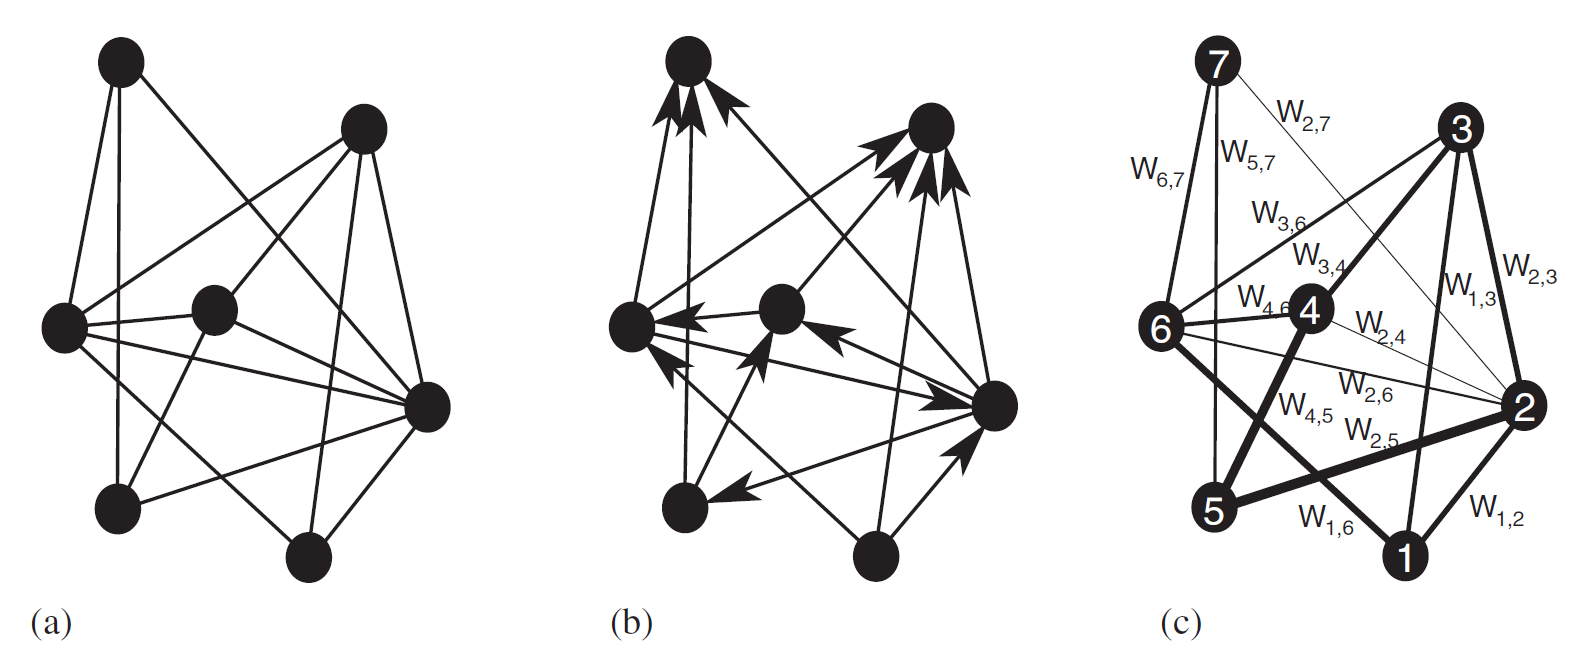
\includegraphics[scale=0.75]{fig/CH2/graph_types_03.PNG}
		\caption{A visual representation of a (a) undirected, (b) directed, and (c) weighted undirected graph, with $N = 7$ and $K = 14$ \citep{boccaletti2006complex}. Typically, the dots represent the nodes and the lines represent the links. The links with the undirected graph has no direction, in contrast with the directed graph, where a direction is indicated. Finally, the links within the undirected weighted graph have an associated weight $w^G_{ij}$. The thickness of the line (link) indicates the weight value assigned to that link. Also, the weight value indicates the degree of connectedness between the nodes.}
		\label{fig:ch2_graph_types}
	\end{center}	
\end{figure}

Now that the necessary notations and definitions are defined, the project can explain how the proposed framework can apply complex network analysis in a fraud prevention context. From here, the term \textit{network analytics} will be used as an umbrella term when referring to an analysis that contains either components of graph theory, social network analysis, or complex network analysis. 

As mentioned before, network analytics has been useful in solving network-related optimisations problems and establishing or quantifying if a relationship exists between the actors in the social network. However, knowing what can be done from network analytics, one needs to ask whether it is an applicable analysis method in a financial fraud context (for example, money laundering) and whether detection systems will benefit from the analysis. \citet{baesens2015fraud} explains the concepts of fraud from a sociological point of view. They explain that if fraud is a social phenomenon, then the concept of \textit{homophily} applies. Homophily is described as the phenomenon where people tend to associate with others whom they perceive as similar to themselves in some way \citep*{newman2018networks}. Therefore, if homophily is applicable, fraudsters will likely associate themselves with other fraudsters due to similar \textit{characteristics} or \textit{behavioural patterns}. 

As mentioned before, one of the steps of a fraud prevention/detection system is to identify emergent patterns that indicate fraudulent or suspicious behaviour (For example, step 1 of phase 2 of the general anti-money laundering process, Figure \ref{fig:ch2_aml_process}). In identifying these patterns, certain characteristic's or behavioural patterns are highlighted, which increases the probability of an event (for example, an account) as being  fraudulent. To illustrate this concept, consider the toy example of two banking clients: Client X is a 54-year-old man that works at an accounting firm and makes an average of 20 wire transfers a month with an average amount of R15 000 per wire transfer. Client Y is a 31-year-old woman that works at a gym and makes an average of 6 wire transfers a month with an average amount of R3 000 per wire transfer. Assuming the bank only had the above data on all their clients, then according to the bank anti-fraud process, it could determine that males above the age of 35 that works for a financial institution and makes more than 15 wire transfers a month of which has an average value more than R10 000 per wire transfer are deemed high risk and could be possible future fraudsters. Therefore, client X will receive a higher fraud risk score than client Y because he fits the profiling better. 

In the example above, the focus should not be the anti-fraud process but the \textit{data} provided to this process. According to the example, the feature's ($\boldsymbol{x}_i$) that the bank had to use to classify the fraud risk (probability of a client being fraudulent in the future - $y_i$) was the age, gender, average number of wire transfers per month, and average value of wire transfers per month of their clients. Currently, the bank is only considering customer information (demographics) and transactional information of the clients. If other dimensions that enrich the existing data are introduced, could this possible improve the risk classification of the existing anti-fraud process? The project proposes that \textit{network analytics} can add these additional dimensions.

If a weighted undirected client network or graph $G^W$ of is constructed at time $t$, denoted as $G^W(t) = (\mathcal{N}_t,\mathcal{L}_t,\mathcal{W}^G_t)$, certain features or metrics can be extracted from the network. In this graph, the links $\mathcal{L}$ represent the transactions connecting the different banking clients, which represent the nodes $\mathcal{N}$. How the weights are assigned to each link in the graph can be done in various ways. 

The type of weight discussed earlier is referred to as a \textit{numeric weight}. As mentioned before, a high value for this type of weight indicates a close affiliation between the nodes. \citet{baesens2015fraud} defined three other types of weights, namely, \textit{binary weight}, \textit{normalised weight}, and \textit{Jaccard weight}. A binary weight is the same as a standard network representation, i.e., the weight value is either 1 or 0  depending on if there is or is not a link present between two nodes, respectively. A normalised weight is a variant of the numeric weight where all the outgoing links weight (assuming we have a directed network) sum up to 1. Finally, the Jaccard weight is a measure of how ``social'' two connected nodes are \citep*{gupte2012measuring}. Formally, the weight $w_ij$ is calculated using the formula $\frac{|\Gamma(n_i) \cap \Gamma(n_j)|} {|\Gamma(n_i) \cup  \Gamma(n_j)|}$, where $\Gamma(n_i)$ and $\Gamma(n_i)$ is the number of events nodes $i$ and $j$ attended. For the current graph, let us assume the weights are defined numerically.       

\citet{baesens2015fraud} mentions that there are three types of analysis techniques in which the main metrics that measure the impact of the social environment on the nodes of interest in a graph are extracted. These techniques and a brief description of each are listed below. 

% Explain each of these!
\begin{enumerate}
    \item \textit{Neighbourhood metrics}: These types of metrics aim to characterise the target of interest-based its direct associates. The \textit{n-order} neighbourhood, nodes that are $n$ ``hops'' away from the node of interest, is used to generate these metrics. The first order ($n = 1$) or \textit{egonet} is commonly used as the selected neighbourhood since scalability issues arise when a $n > 1$ neighbourhood is chosen in large networks.   
    \item \textit{Centrality metrics}: These measures try to quantify an individual's importance in a social network \citep{boccaletti2006complex}. Typically, centrality metrics consider the entire network structure or subgraph when measures are extracted. 
    \item \textit{Collective inference algorithms}: This analysis technique is essential for propagating or diffusing information through the network. For example, if we have a network where only certain nodes (banking clients) are labelled to be money launderers and others legitimate.  Fraud analysis can use collective inference algorithms to infer a probability that an unlabelled node is more likely to be a  money launderer or legitimate client based on the known information of the graph. Using the previous example, as opposed to neighbourhood and centrality metrics, collective inference algorithms compute the probability that a node is exposed to money laundering activity and quantify the ``influence'' the criminal act has on the unlabeled nodes.    
\end{enumerate}

Table \ref{tab:ch2_sna_metrics}summarises the most commonly used metrics derived using the above three analysis methods. The definitions and notation of each of the table's metrics were primarily obtained by \citet{boccaletti2006complex, baesens2015fraud,} and \citet*{humpherys2017foundations}. In addition, there are other network metrics mentioned, such as link density, clustering coefficient, modularity, motifs, and efficiency. However, we will primarily focus on the metrics mentioned in Table \ref{tab:ch2_sna_metrics} for the project. 

Returning to our weighted undirected client network or graph $G^W(t)$, where the nodes represent the banking clients, and the links represent the transactions made by the clients, we have established that it will be possible to extract network metrics from this graph that could give insight into  a clients influence ability, connectives, importance, etc. The previous section established that machine learning is the main field dedicated to the broad premise of learning from data and that several learning paradigms were developed to act as a framework to encapsulate this premise. As mentioned before, supervised learning is the learning type that is the paper's main focus since it aims to predict the probability that a banking client will commit money laundering in the future using a set of defined input features. A critical question that the paper needs to consider is if including the network metrics as inputs to the supervised model will increase the model's overall performance? This question is posed due to the possibility of presenting the classification model with the adjacency matrix, in vector form $\bold{a} = \{a_{1,1}, a_{1,2}, \ldots, a_{n,n} \}$, as an input feature, along with the other useful input features. If the classifier is optimal, then it would be able to detect any class of patterns, and it would be able to describe the system as a network, then the exercises of building a network and extracting network metrics would be meaningless. \citet*{zanin2016combining} asked the same question and illustrated with a numeric experiment how this hypothesis is easily disproved. In short, for \textit{part one} of the experiment, they sampled 20 000 random networks, each having $N = 10$ and a link density of 0.3. Then two topological metrics, efficiency and clustering coefficient, were extracted from each network. For \textit{part two} of the experiment, they input the adjacency matrices of the sampled networks to an artificial neural network trained to recover the obtained metric values. For the \textit{third part} of the experiment, they linearly fitted both values (the true topological values and estimated values produced by the artificial neural network) and calculated the coefficient of determination $R^2$ for a range of different hidden neurons. In each case, the $R^2$ value obtained was minimal ($<0.04$), proving that the model could not recover the true topological metrics. \citet{zanin2016combining} mentioned that the goal of the simple numeric experiment was to illustrate that a single learning algorithm is not sufficient to deal with the structure of a complex system. Therefore, the complex network approach adds important value to the study of complex systems, which cannot be obtained by machine learning alone. \citet{zanin2016combining} concluded by saying that it is possible that complex network analysis and machine learning can be used synergistically and gives examples where researchers used machine learning and complex networks to create classification models in the biomedical and engineering fields. 

In conclusion to this chapter, the project will aim to provide evidence that supports the findings of \citet{zanin2016combining} - that combining complex network analysis and machine learning, better money laundering classifiers can be constructed. This chapter formed a critical part in the project since, firstly, adequate knowledge of the problem - money laundering needed to be established. Therefore, understanding the money laundering process and its known forms is essential for the solution generating process. Secondly, understanding the existing techniques in which money laundering is combated (anti-money laundering processes) is essential for the project purpose (that could provide insight into improving anti-money laundering processes). And finally, introducing both machine learning and complex network analysis and how they can be used synergistically to produce stronger, more robust classification models. The next chapter will discuss the methodology implemented to test the projects hypothesis.     


% Please add the following required packages to your document preamble:
% \usepackage{multirow}
\begin{sidewaystable}
\begin{adjustbox}{scale=0.65,center}
\begin{tabular}{ccll}
\hline
\textbf{Analysis technique}                                                      & \textbf{Metric}                                                                                    & \multicolumn{1}{c}{\textbf{Short description of metric}}                                                                                                                                                                                                                                                                                                                                                                                                                                                                                                                                                                                                       & \multicolumn{1}{c}{\textbf{Formula to caculate metric or metric symbol}}                                                                                                                                                                                                                                                                                                                                                                                                                                                                                               \\ \hline
\multirow{7}{*}{\begin{tabular}[c]{@{}c@{}}Neighborhood \\ metrics\end{tabular}} & \multicolumn{1}{c|}{Degree}                                                                        & \multicolumn{1}{l|}{\begin{tabular}[c]{@{}l@{}}The degree $k_i$ of node $i$ is the number\\ of links incident with the node.\end{tabular}}                                                                                                                                                                                                                                                                                                                                                                                                                                                                                                                     & $k_i = \sum_{j \in \mathcal{N}}^{}a_{ij}$                                                                                                                                                                                                                                                                                                                                                                                                                                                                                                                              \\ \cline{2-4} 
                                                                                 & \multicolumn{1}{c|}{Traingle}                                                                      & \multicolumn{1}{l|}{\begin{tabular}[c]{@{}l@{}}The number of cycles ($C_k$) that has $k = 3$\\  of  which node $i$ forms part of.\end{tabular}}                                                                                                                                                                                                                                                                                                                                                                                                                                                                                                                & $triangle(n_i)$                                                                                                                                                                                                                                                                                                                                                                                                                                                                                                                                                        \\ \cline{2-4} 
                                                                                 & \multicolumn{1}{c|}{Density}                                                                       & \multicolumn{1}{l|}{\begin{tabular}[c]{@{}l@{}}The density of a graph is the ratio of the number of edges \\ and a number of possible edges. This measure\\ indicates how ``connected'' nodes in a network are to \\ each other.\end{tabular}}                                                                                                                                                                                                                                                                                                                                                                                                                 & $p(G) = \frac{2K}{N(N-1)}$                                                                                                                                                                                                                                                                                                                                                                                                                                                                                                                                             \\ \cline{2-4} 
                                                                                 & \multicolumn{1}{c|}{Strength}                                                                      & \multicolumn{1}{l|}{\begin{tabular}[c]{@{}l@{}}The sum of the weights of each edge adjacent \\ to a vertex. Also known as the degree strength.\end{tabular}}                                                                                                                                                                                                                                                                                                                                                                                                                                                                                                   & \begin{tabular}[c]{@{}l@{}}$s_i = \sum_{j=1}^{N}a_{ij}w^G_{ij}$\\ Where $s_i$ is the degree strength of node $i$.\end{tabular}                                                                                                                                                                                                                                                                                                                                                                                                                                         \\ \cline{2-4} 
                                                                                 & \multicolumn{1}{c|}{\begin{tabular}[c]{@{}c@{}}Transitivity \\ (local)\end{tabular}}               & \multicolumn{1}{l|}{\begin{tabular}[c]{@{}l@{}}Measures the probability that \\ adjacent vertices of a vertex are connected.\\ The measure is also known as the \\ \textit{clustering coefficient}.\end{tabular}}                                                                                                                                                                                                                                                                                                                                                                                                                                              & \begin{tabular}[c]{@{}l@{}}$C^W_i = \frac{1}{s_i(k_i-1)}\sum_{j,h}\frac{w^G_{ij}+w^G_{ih}}{2}a_{ij}a_{ih}a_{jh}$\\ Where $C^W_i$ provides the locally weighted transitivity of node $i$.\end{tabular}                                                                                                                                                                                                                                                                                                                                                                  \\ \cline{2-4} 
                                                                                 & \multicolumn{1}{c|}{\begin{tabular}[c]{@{}c@{}}Relational \\ neighbour\end{tabular}}               & \multicolumn{1}{l|}{\begin{tabular}[c]{@{}l@{}}The relative number of neighbours that is allocated\\ to a specific class, for example, a neighbourhood node can \\ have the label HC that indicates that they are an honest \\ client or they can have the label MLC, which indicate that\\ the client is a money-laundering client.\end{tabular}}                                                                                                                                                                                                                                                                                                             & \begin{tabular}[c]{@{}l@{}}$P(class|n_i) = \frac{1}{Z}\sum_{n_j \in {Neighbourhood_n}_i} w^G_{ij}$\\ Where $Z$ is a normalisation factor, ${Neighbourhood_n}_i$ is the\\ $1^{st}$ degree neighbourhood of node $i$, and $class$ is the label \\ of interest.\end{tabular}                                                                                                                                                                                                                                                                                              \\ \cline{2-4} 
                                                                                 & \multicolumn{1}{c|}{\begin{tabular}[c]{@{}c@{}}Probabilistic \\ relational neighbour\end{tabular}} & \multicolumn{1}{l|}{\begin{tabular}[c]{@{}l@{}}This metric is an extension of the relational neighbour\\ metric, whereas the weight, $w^G_{ij}$ is defined\\ as the probability of node $j$ (a neighbour of node $i$)\\ belonging to a certain class. For example,  the probability \\ of node $n_i$ being a money-laundering client is equal\\ to the sum of the probabilities of neighbouring nodes, \\ which are classified as money launderers.\end{tabular}}                                                                                                                                                                                              & \begin{tabular}[c]{@{}l@{}}$P(class|n_i) = \frac{1}{Z}\sum_{n_j \in {Neighbourhood_n}_i} w^G_{ij}$\\ Where $w^G_{ij} = P(class|n_j)$.\end{tabular}                                                                                                                                                                                                                                                                                                                                                                                                                      \\ \cline{2-4} 
\multirow{5}{*}{\begin{tabular}[c]{@{}c@{}}Centrality \\ metrics\end{tabular}}   & \multicolumn{1}{c|}{Geodesic path}                                                                 & \multicolumn{1}{l|}{The walk that has the smallest length between nodes.}                                                                                                                                                                                                                                                                                                                                                                                                                                                                                                                                                                                      & $min(d(n_i,n_j))$                                                                                                                                                                                                                                                                                                                                                                                                                                                                                                                                                      \\ \cline{2-4} 
                                                                                 & \multicolumn{1}{c|}{\begin{tabular}[c]{@{}c@{}}Closeness \\ centrality\end{tabular}}               & \multicolumn{1}{l|}{\begin{tabular}[c]{@{}l@{}}The average distance from node $i$ to all other nodes\\ in the graph. Closeness centrality is the reciprocal\\ of \textit{farness}.\end{tabular}}                                                                                                                                                                                                                                                                                                                                                                                                                                                               & \begin{tabular}[c]{@{}l@{}}$c(n_i) = \left [\frac{\sum_{j=1;j\neq i}^{N}d(n_i,n_j)}{N-1}\right ]^{-1}$\\ Very large values of $d(n_i,n_j)$ are often excluded due to $\lim_{x \to -\infty}\left (\frac{1}{x} \right )$.\end{tabular}                                                                                                                                                                                                                                                                                                                                    \\ \cline{2-4} 
                                                                                 & \multicolumn{1}{c|}{\begin{tabular}[c]{@{}c@{}}Eigenvector \\ centrality\end{tabular}}             & \multicolumn{1}{l|}{\begin{tabular}[c]{@{}l@{}}The eigenvector centrality score corresponds to the  \\ values of the first eigenvector of the graph adjacency matrix. \\ Therefore, it measures the importance of nodes in a \\ network using the adjacency and eigenvector matrices.\end{tabular}}                                                                                                                                                                                                                                                                                                                                                            & \begin{tabular}[c]{@{}l@{}}$\Upsilon \vec{C_{\mathrm{IV}}}=\boldsymbol{A}\vec{C_{\mathrm{IV}}}$\\ Where $\vec{C_{\mathrm{IV}}}$ is the eigenvector, and $\Upsilon$ the eigenvalue.\end{tabular}                                                                                                                                                                                                                                                                                                                                                                        \\ \cline{2-4} 
                                                                                 & \multicolumn{1}{c|}{Betweenness}                                                                   & \multicolumn{1}{l|}{\begin{tabular}[c]{@{}l@{}}The betweenness metric counts the number times a\\ node lies on the geodesic between any two nodes\\ in the network graph.\end{tabular}}                                                                                                                                                                                                                                                                                                                                                                                                                                                                        & \begin{tabular}[c]{@{}l@{}}$b(n_i) = \sum_{j\neq h \neq i}^{}\frac{g_{jh}(n_i)}{g_{jh}}$\\ Where $g_{jh}$ is the total number of shortest paths from \\ node $j$ to node $h$ and  $g_{jh}(n_i)$ is the number of \\ those paths that pass through node $i$.\end{tabular}                                                                                                                                                                                                                                                                                               \\ \cline{2-4} 
                                                                                 & \multicolumn{1}{c|}{Graph theoretic center}                                                        & \multicolumn{1}{l|}{\begin{tabular}[c]{@{}l@{}}The node with the smallest maximum distance to\\ all other nodes in the network.\end{tabular}}                                                                                                                                                                                                                                                                                                                                                                                                                                                                                                                  & \begin{tabular}[c]{@{}l@{}}$G_{centre} = min(max(path(n_i,n_j)))$\\ Where $path(n_i,n_j)$ gives the length of the path(s)\\ from node $i$ to $j$ and $\{i,j = \{1,2, \ldots, N \}, i \neq j\}$.\end{tabular}                                                                                                                                                                                                                                                                                                                                                           \\ \cline{2-4} 
\begin{tabular}[c]{@{}c@{}}Collective inference \\ algorithms\end{tabular}       & \multicolumn{1}{c|}{PageRank}                                                                      & \multicolumn{1}{l|}{\begin{tabular}[c]{@{}l@{}}The PageRank algorithm is an algorithm that ranks the\\ nodes in a graph by some importance. The PageRankalgorithm forms \\ the basis of Google's search engine algorithm for ranking web pages. \\ Using web pages as an example, the algorithm determines the probability \\ of a web surfer visiting a  specific web page. The probability of visiting a \\ web page is called its pagerank. Referring to the above example, PageRank \\ can establish the propagation of page influence through the network. \\ Similarly, the algorithm can be used to propagate fraud throughout a network.\end{tabular}} & \begin{tabular}[c]{@{}l@{}}$\bold{p}(0) = \frac{1}{N}\bold{1}$;\\ $\bold{p}(t+1) = \alpha(D^{-1}\bold{A})^T\bold{p}(t) + \frac{1-d}{N}\bold{1}$\\ Where $\bold{p}(t) = \{p_1(t), \{p_2(t), \ldots, \{p_N(t)\}^T$, \\ $\bold{1}$ is a vector of $N$ ones, $D$ is a diagonal matrix, \\ and $\alpha$ is the damping factor\footnote{The expression is in matrix form. Also, the expression is the modified version of the original PageRank expression. This version accounts for pages with no outbound links and incorporates the boredom factor.}.\end{tabular} \\ \cline{2-4} 
\end{tabular}
\end{adjustbox}
\caption{Summary of the main metrics produced by the three types of analysis techniques used to analyse the social environment of nodes in a graph:  i) neighbourhood metrics, ii) centrality metrics, and iii) inference algorithms. The metrics produced by each analysis technique is given along with a short description of the metric and an expression used to calculate the metric.}
\label{tab:ch2_sna_metrics}
\end{sidewaystable}










